\graphicspath{{./background/}}

\chapter{Background}
% {{{
\label{chap:background}

%TODO: mention that this chapter will not be discussing compression specific
%background

Information visualisation techniques are very domain specific; one type of
visualisation may work well for a specific scenario, but it will work quite
poorly when applied to another domain. The problem domain applicable to this
project is the effective visualisation of point cloud data, more specifically,
water molecules from molecular simulations. Some of the important issues that
will be need to be investigated will be the level of detail chosen and how
easily it will be to see what is happening, such as interactions or object
relationships.

Section \ref{sec:molecularvis} will identify and briefly introduce several
molecular visualisation techniques. While Section \ref{sec:generalvis} will
focus on more general visualisation techniques.


\section{Molecular visualisation}
% {{{
\label{sec:molecularvis}

The most significant problem for visualising molecular data is the amount of
data available and how to represent them so as not to clutter up the display.
Some of the molecular visualisation techniques focuses on simplifying the
models, by analysing the data to identify structures; while some exclude
certain data from the visualisation. Either way, a more simplified image is
presented so as to make it easier and quicker to understand.

The more specific visualisation techniques (ribbon, paper chain and twister) are
designed for very specific molecular objects, thus they will not be easily
extendable to point cloud data. They can however be used to see what kind of
analysis can be done on data to simplify and help identify structures.

It is worth mentioning the Visual Molecular Dynamics (VMD) \citep{humphrey96}
program, which is a commonly used visualisation package aimed at displaying,
animating and analysing large biomolecular systems \citep{VMD}. However, as VMD
is aimed at general biomolecular systems, the support for specific
visualisation and filtering is limited. VMD does support and use some of the
visualisation techniques that will be mentioned later in this section.

\subsection{Ball-and-stick}
% {{{
\label{sub:ball_stick}

The ball-and-stick model is the classical approach to displaying molecular
structure. Colour coded spheres are used to represent the atoms, while
cylinders are used to represent the bonds between them (see figure
\ref{fig:ballstick} for an example image). This model is used to emphasise the
molecular connectivity of the atoms. This is the simplest of approaches to
molecular visualisation and is also used when all the detail is required,
typically for looking at bond information and reaction sites.

The problem with this model is that it does not handle large numbers of atoms
and bonds very well. By having all the atoms and bonds visible, the image
quickly becomes crowded and overall structure is obscured. Occlusion of other
atoms often occurs which may hide important information. Ball-and-stick diagrams
are typically not used for large or many molecules as it typically produces the
most cluttered diagrams, making it very difficult to understand and analyse.

\begin{figure}[h!]
  \begin{center}
    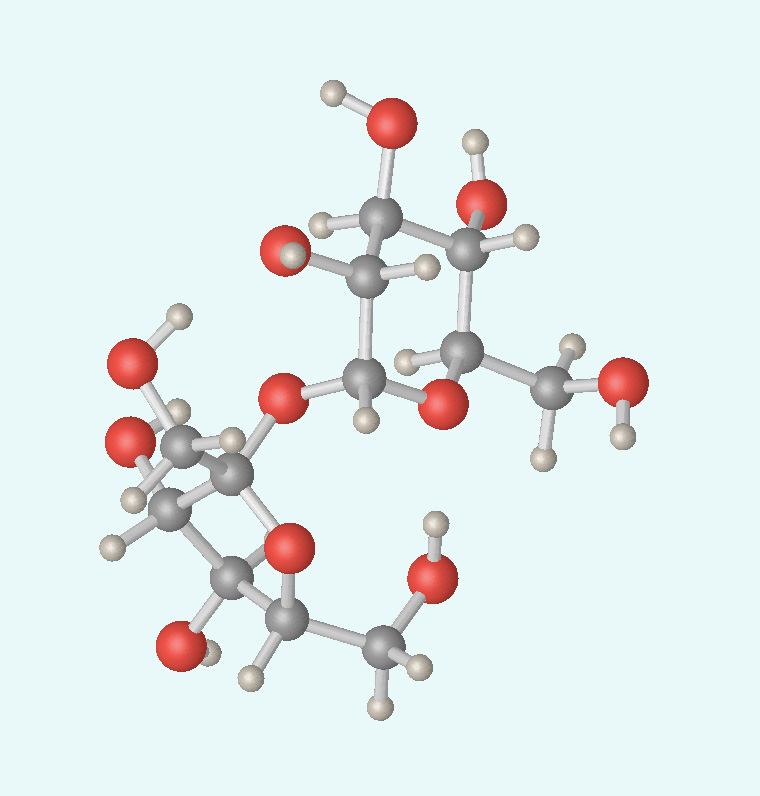
\includegraphics[width=70mm]{BallStick}
  \end{center}
  \caption{A typical ball-and-stick model}
  \label{fig:ballstick}
\end{figure}

% }}}

\subsection{CPK}
% {{{
\label{sub:cpk}

The CPK (Corey-Pauling-Koltun) \citep{corey53} representation simplifies the
ball-and-stick model by doing away with cylinders for bonds; instead, the
spheres used for the atoms are enlarged to encompass the bonds. The atoms now
overlaps with one another, covering up where the bonds would be (see figure
\ref{fig:cpk}).

Removing the bonds from the model representation simplifies the display and
allows for the overall shape and contour to be easily seen. Although this model
has simplified the ball-and-stick model, it does not highlight any structures,
it has only removed the bond information. The later molecular visualisation
techniques in this paper do highlight certain molecular structures.

The CPK representation also suffers from not being able to visualise large
numbers of molecules. As each of the atoms has been enlarged, each molecule
essentially occupies more space than the ball-and-stick model; with the
molecules being opaque, this causes large areas to be occluded from sight, which
may hide important information and make it hard to analyse an entire system.

\begin{figure}[h!]
  \begin{center}
    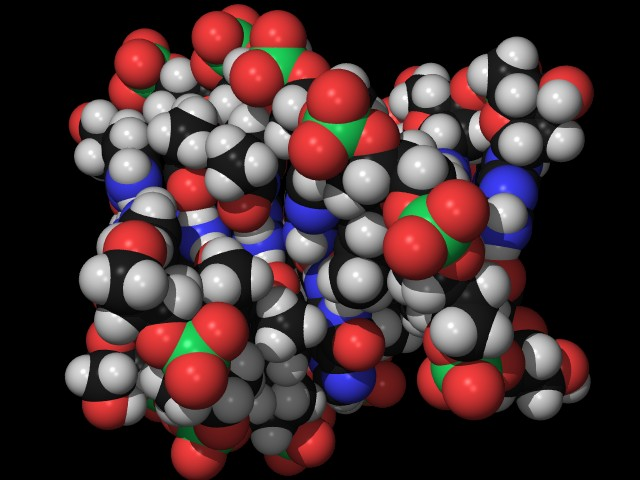
\includegraphics[width=70mm]{CPK-big}
  \end{center}
  \caption{CPK}
  \label{fig:cpk}
\end{figure}

% }}}

\subsection{Protein molecules}
% {{{
\label{sub:protein}

The ribbon model (\citep{richardson81}, \citep{carson87}) was designed to
highlight the structure of protein molecules by fitting a curved surface to the
backbone of the molecule. This allows for the shape of the protein molecule to
be easily seen and followed (see figure \ref{fig:ribbon}).

This proved to be highly effective at highlighting the structure of proteins;
unfortunately this approach is not as effective when applied to non-protein
molecules such as carbohydrates and lipids, where the molecular structure is
different. Thus, the traditional ball-and-stick and CPK models do still get
used for carbohydrate and lipid molecules.

\begin{figure}[h!]
  \begin{center}
    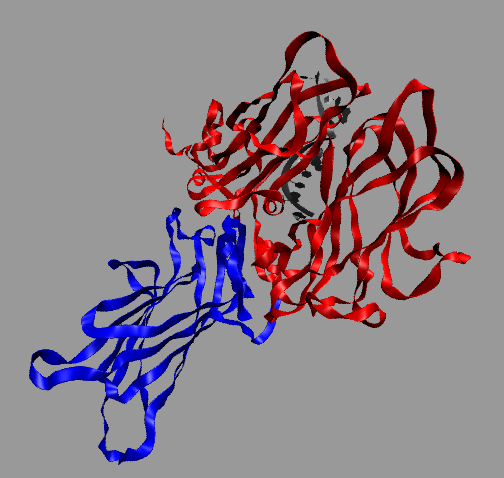
\includegraphics[width=70mm]{ribbon}
  \end{center}
  \caption{Ribbon}
  \label{fig:ribbon}
\end{figure}

% }}}

\subsection{Carbohydrate molecules}
% {{{
\label{sub:carbohydrate}

The paper chain visualisation technique \citep{kuttel06} focuses on highlighting
ring structures in carbohydrate molecules. Ring structures are first identified
and then are displayed using a ring polyhedron (see figure \ref{fig:paperchain}).

This significantly simplifies the carbohydrate molecules by only showing the
carbohydrate rings, which would of otherwise been obscured by the other
visualisations (ball-and-stick and CPK). The ball-and-stick model can still be
overlayed on the paper chain diagram to provide detailed information if needed.

\begin{figure}[h!]
  \begin{center}
    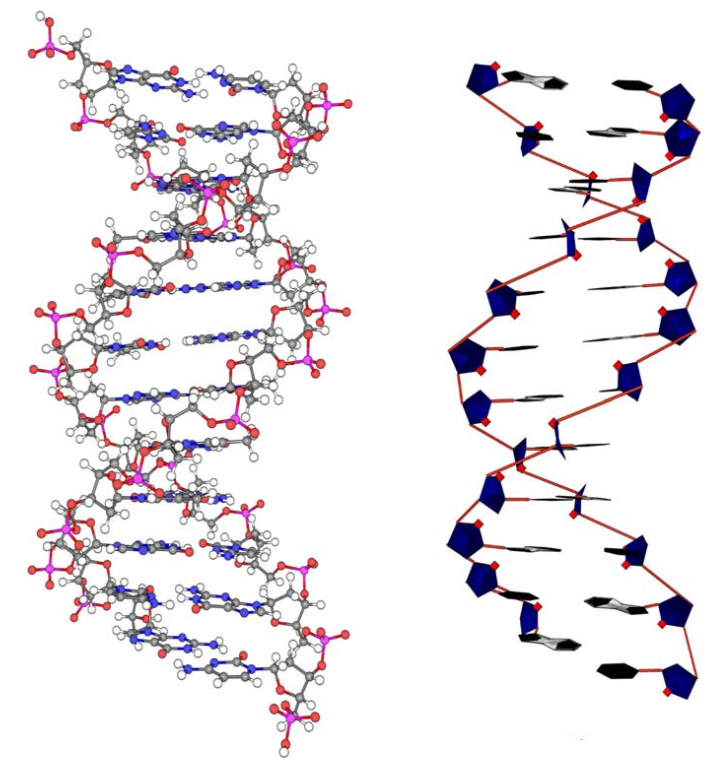
\includegraphics[width=70mm]{paper_chain}
  \end{center}
  \caption{Paper chain}
  \label{fig:paperchain}
\end{figure}

The twister visualisation technique \citep{kuttel06} builds on the paper
chain technique by highlighting the relative orientations of the identified
carbohydrate rings. Each carbohydrate ring is represented by a disc, which is
then connected to another disc with a ribbon. The ribbon will follow the
orientation from one ring to another, thus showing how the rings are connected
to one another (see figure \ref{fig:twister}).

This is similar to the ribbon model for proteins in that it shows the overall
shape of the molecule quite effectively. However, like the ribbon model, this
visualisation technique is designed for a specific type of molecule;
carbohydrates for the twister technique.

\begin{figure}[h!]
  \begin{center}
    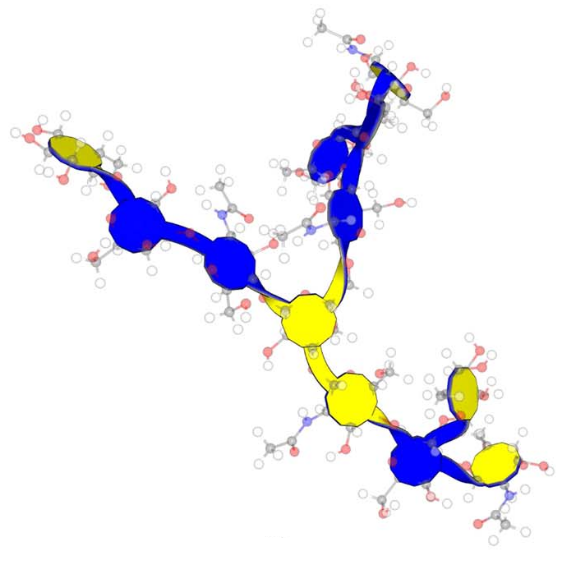
\includegraphics[width=70mm]{twister}
  \end{center}
  \caption{Twister}
  \label{fig:twister}
\end{figure}

% }}}

% }}}

\section{General visualisation}
% {{{
\label{sec:generalvis}

More research has been completed for general data visualisation techniques than
that of molecular visualisations. The most relevant areas of research to point
cloud visualisation are: volume visualisation and clutter reduction. Both of
which will be briefly introduced in this section.

Traditional volume visualisation techniques work on volumes of data, such as
data from CT and MRI scans. The main approaches to visualising such data would
be surface extraction, for finding the shape of the volume; and volume
rendering, rendering the volume such that the volume in its entirety is
visible.

This paper will only mention the basic different techniques and will not provide
much detail on the individual algorithms. There has also been significant
advances in each of the techniques \citep{brodlie01}, which will not be
mentioned in this paper.

\subsection{Surface extraction}
% {{{
\label{sub:surface_extraction}

Surface extraction is used to determine the surfaces of volume data. The
marching cubes algorithm \citep{lorensen87} is the classical approach for
surface extraction. The algorithm works by examining each cell in the data (a
cube) and determining whether it is inside the volume or not. A surface can
then be determined by combining all the cells which intersect with the volume
boundary (see figure \ref{fig:triangulatedmesh}).

Surface extraction allows for the shape of the volume to be extracted and be
easily seen, this is somewhat analogous to the CPK model in that regard.
Surface extraction can be adapted to molecular data to provide a simpler and
smoothed view of the molecule, so that the shape and contours can be more
plainly seen; which may of otherwise been obscured by the individual atoms.
Conversely, this technique can also be used to identify volumes of space where
points are missing, thus highlighting these areas instead.

\begin{figure}[h!]
  \begin{center}
    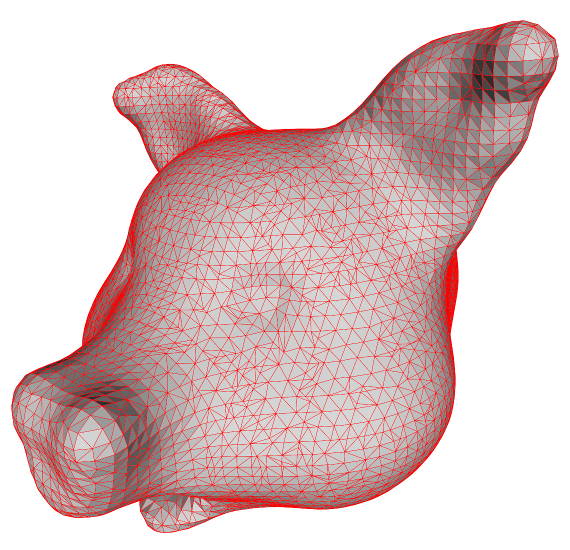
\includegraphics[width=70mm]{triangulated_mesh}
  \end{center}
  \caption{Surface extraction}
  \label{fig:triangulatedmesh}
\end{figure}

% }}}

\subsection{Volume rendering}
% {{{
\label{sub:volume_rendering}

Volume rendering aims to visualise the entire volume instead of a subset. This
is done by modelling the data as a translucent gel so that you are able to see
through the volume, while still being able to see what is in the volume at the
same time (see figure \ref{fig:headvolume}).

There are two main approaches to volume rendering; the first is working from the
image plane to the volume, this is called image order processing. Ray casting is
the classical approach to this as proposed by \citet{levoy88}. Object order
processing is working from the volume to the image plane. The classical approach
to this is splatting \citep{westover89}. Hybrid methods have been developed to
take advantage of both approaches.

The advantage of volume rendering is being able to visualise the entire volume
at once, but does come at the cost of increased complexity and computation.
While volume rendering will not be directly applicable to molecular data as the
requirement is often to see the individual atoms or structures, rather than an
aggregated view of the entire volume data.

However, volume rendering could be useful for seeing what a volume looks like
or behaves at a glance. For simulations where large parts of the volume are
homogenous (e.g. filled with water), volume rendering could be useful for
visualising these homogenous volumes.

\begin{figure}[h!]
  \begin{center}
    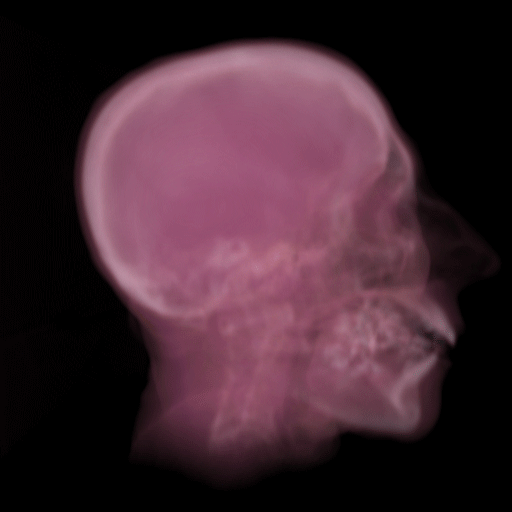
\includegraphics[width=70mm]{head_volume}
  \end{center}
  \caption{Volume rendering}
  \label{fig:headvolume}
\end{figure}

% }}}

\subsection{Metaballs}
% {{{
\label{sub:metaballs}

%TODO: get references to metaballs and solvent accessible surfaces

Metaballs is a technique for producing organic-looking objects (see figure
\ref{metaballs}). A metaball is modelled after a number of points which exerts
a force around it, the surface of the metaball is the set of points where the
force function is equal to some constant threshold value. The surface is
usually determined using surface extraction techniques.

The advantage of metaballs is that volume data is grouped together, making it
easy to see the different volumes in an area. The disadvantage of this
technique is the computation cost required to determine and extract the surface
from the force calculations.

\begin{figure}[h!]
  \begin{center}
    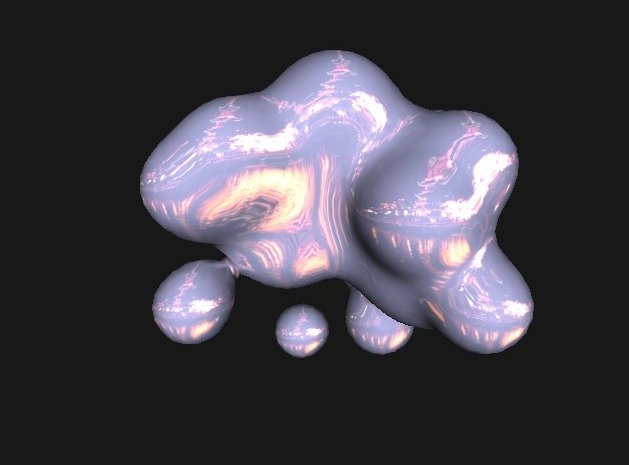
\includegraphics[width=70mm]{metaballs}
  \end{center}
  \caption{Metaballs}
  \label{fig:metaballs}
\end{figure}

Solvent accessible surface rendering for molecular modelling produces a similar
effect to metaballs. The difference is the approach taken to produce the
surface of the volume. Solvent accessible surface rendering creates a surface
by determining the surface where the solvent (modelled with spheres) cannot
fit. See figure \ref{fig:sas}.

\begin{figure}[h!]
  \begin{center}
    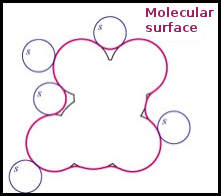
\includegraphics[width=70mm]{sas_ms}
  \end{center}
  \caption{Solvent accessible surface}
  \label{fig:sas}
\end{figure}

% }}}

\subsection{Clutter reduction}
% {{{
\label{sub:clutter_reduction}

Shneiderman provides a visual information-seeking mantra \citep{shneiderman96}:
``overview first, zoom and filter, then details on demand'', in which clutter
reduction techniques fit in quite well. The mantra provides a general hierarchy
of tasks that is to be applied to information visualisation, in which clutter
reduction plays an important role.

\citet{ellis07} provides a taxonomy containing many clutter reduction techniques
against many criteria. With clutter reduction, a balance between removing too
much and too little information must be made. Removing too much or too little
data will make the visualistion of little use.

With regards to visualising point cloud data, filtering, opacity and topological
distortion may be the most useful clutter reduction techniques.

Filtering is only displaying certain items fulfilling a criteria. This can be
used to only show items in a certain area or locus of interest, irrelevant items
can be removed and not clutter up the display. This may be useful for removing
uninterested in occluding objects and only show points at important areas, such
at where there is interaction occurring.

Another approach to filtering is to highlight the important features of the
data with colour, but leave the rest of the data visible as is. This adds the
advantage of keeping context data. Figure \ref{fig:graphhighlight} is an
example application of highlighting in a graph structure.

Opacity is changing the translucency of items to highlight or hide things. This
is similar to filtering in that irrelevant items are partially or entirely
hidden, highlighting only the important parts. The advantage of opacity over
filtering is that the other information is not entirely removed, it is still
available if needed and can be used to hint at contextual information. Opacity
can also be adapted to show temporal information, where the previous frame is
rendered along with the current frame, but at a lower opacity; creating an
effect similar to motion blur.

Topological distortion is changing the view so that certain areas are larger.
Thus highlighting and bringing to focus the relevant area, while de-emphasising
the other areas. The distortion can either be uniform (zooming), or can be
non-uniform (fish-eye effect).

Clutter reduction techniques has the most potential for point cloud
visualisation as there is a need to be able to visualise many objects in 3D
space, however care must be taken to not remove important and relevant
information. It should be noted that the clutter reduction techniques are not
all mutually exclusive, many of the techniques can be used to complement and be
layered on top of one another.

\begin{figure}[h!]
  \begin{center}
    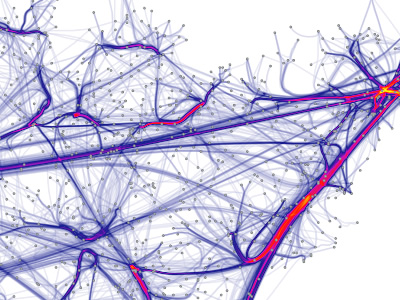
\includegraphics[width=70mm]{graph_highlight}
  \end{center}
  \caption{Highlighting}
  \label{fig:graphhighlight}
\end{figure}

% }}}

% }}}

This paper has gone through some visualisation techniques, each with their own
advantages and disadvantages. Visualisation techniques are all quite specific
and are designed for their respective scenarios, fulfilling their respective
requirements and taking advantage of specific domain knowledge; as a result,
they are not easily generalisable into other areas.

Molecular modelling is a specific instance of the information visualisation
problem, where the requirement is to be able to easily identify certain
structures. Different types of molecules will each have their own specific
characteristics and structures, this knowledge can be taken advantage of in the
different visualisation techniques: ribbon diagrams are useful for proteins,
paper chain and twister for carbohydrates, while ball-and-stick and CPK for
general molecular visualisations.

General visualisation techniques address a slightly different problem; the
problem being solved is how to be able to visualise the data effectively and
not necessarily to identify and highlight certain structures. Identifying the
structures is often domain specific and thus approaches are not easily
extendable to their domains, thus the main concern is how to enable easy
exploration of the data.

None of the techniques touched on, handle a temporal aspect explicitly. If a
temporal dimension were to be added, all the techniques would just treat each
frame separately and regenerate the visualisation given the new set of data.
This approach would not be ideal if some inter-frame visualisation coherence is
desired. This aspect in information visualisation is quite lacking and thus ways
of visualising temporal information will need to be developed.

There is no one solution for all visualisation needs, however approaches and
ideas can be taken from different visualisation areas. Although the problems
may not be identical, there will be some overlapping requirements and concerns.
As mentioned in the introduction, visualisation techniques are very domain
specific, with their own requirements and concerns.

% }}}

